% Options for packages loaded elsewhere
\PassOptionsToPackage{unicode}{hyperref}
\PassOptionsToPackage{hyphens}{url}
%
\documentclass[
]{book}
\title{Geography in the Field II: Mapping London}
\author{Justin van Dijk}
\date{2022-01-19}

\usepackage{amsmath,amssymb}
\usepackage{lmodern}
\usepackage{iftex}
\ifPDFTeX
  \usepackage[T1]{fontenc}
  \usepackage[utf8]{inputenc}
  \usepackage{textcomp} % provide euro and other symbols
\else % if luatex or xetex
  \usepackage{unicode-math}
  \defaultfontfeatures{Scale=MatchLowercase}
  \defaultfontfeatures[\rmfamily]{Ligatures=TeX,Scale=1}
\fi
% Use upquote if available, for straight quotes in verbatim environments
\IfFileExists{upquote.sty}{\usepackage{upquote}}{}
\IfFileExists{microtype.sty}{% use microtype if available
  \usepackage[]{microtype}
  \UseMicrotypeSet[protrusion]{basicmath} % disable protrusion for tt fonts
}{}
\makeatletter
\@ifundefined{KOMAClassName}{% if non-KOMA class
  \IfFileExists{parskip.sty}{%
    \usepackage{parskip}
  }{% else
    \setlength{\parindent}{0pt}
    \setlength{\parskip}{6pt plus 2pt minus 1pt}}
}{% if KOMA class
  \KOMAoptions{parskip=half}}
\makeatother
\usepackage{xcolor}
\IfFileExists{xurl.sty}{\usepackage{xurl}}{} % add URL line breaks if available
\IfFileExists{bookmark.sty}{\usepackage{bookmark}}{\usepackage{hyperref}}
\hypersetup{
  pdftitle={Geography in the Field II: Mapping London},
  pdfauthor={Justin van Dijk},
  hidelinks,
  pdfcreator={LaTeX via pandoc}}
\urlstyle{same} % disable monospaced font for URLs
\usepackage{longtable,booktabs,array}
\usepackage{calc} % for calculating minipage widths
% Correct order of tables after \paragraph or \subparagraph
\usepackage{etoolbox}
\makeatletter
\patchcmd\longtable{\par}{\if@noskipsec\mbox{}\fi\par}{}{}
\makeatother
% Allow footnotes in longtable head/foot
\IfFileExists{footnotehyper.sty}{\usepackage{footnotehyper}}{\usepackage{footnote}}
\makesavenoteenv{longtable}
\usepackage{graphicx}
\makeatletter
\def\maxwidth{\ifdim\Gin@nat@width>\linewidth\linewidth\else\Gin@nat@width\fi}
\def\maxheight{\ifdim\Gin@nat@height>\textheight\textheight\else\Gin@nat@height\fi}
\makeatother
% Scale images if necessary, so that they will not overflow the page
% margins by default, and it is still possible to overwrite the defaults
% using explicit options in \includegraphics[width, height, ...]{}
\setkeys{Gin}{width=\maxwidth,height=\maxheight,keepaspectratio}
% Set default figure placement to htbp
\makeatletter
\def\fps@figure{htbp}
\makeatother
\setlength{\emergencystretch}{3em} % prevent overfull lines
\providecommand{\tightlist}{%
  \setlength{\itemsep}{0pt}\setlength{\parskip}{0pt}}
\setcounter{secnumdepth}{5}
\usepackage{booktabs}
\usepackage{amsthm}
\makeatletter
\def\thm@space@setup{%
  \thm@preskip=8pt plus 2pt minus 4pt
  \thm@postskip=\thm@preskip
}
\makeatother
\ifLuaTeX
  \usepackage{selnolig}  % disable illegal ligatures
\fi
\usepackage[]{natbib}
\bibliographystyle{plainnat}

\begin{document}
\maketitle

{
\setcounter{tocdepth}{1}
\tableofcontents
}
\hypertarget{section}{%
\chapter*{}\label{section}}
\addcontentsline{toc}{chapter}{}

\hypertarget{why-london}{%
\section*{Why London?}\label{why-london}}
\addcontentsline{toc}{section}{Why London?}

It is an exciting time to be a quantitative geographer in London. The city is generating more data for us to work with than ever before. Maps, graphics and infographics about the city are everywhere more people live here than at any time in London's history. A great example of the variety of data that is available for London is captured in the book {[}London: The Information Capital{]} by \href{https://jcheshire.com/}{James Cheshire} and \href{https://www.oliveruberti.com/the-information-capital}{Oliver Uberti}. As geographers, we are in a critical position both to be able to capitalise on these developments for our own research but also view them a little more critically than others who have not had the benefit of decades of social and spatial research.

\begin{figure}

{\centering 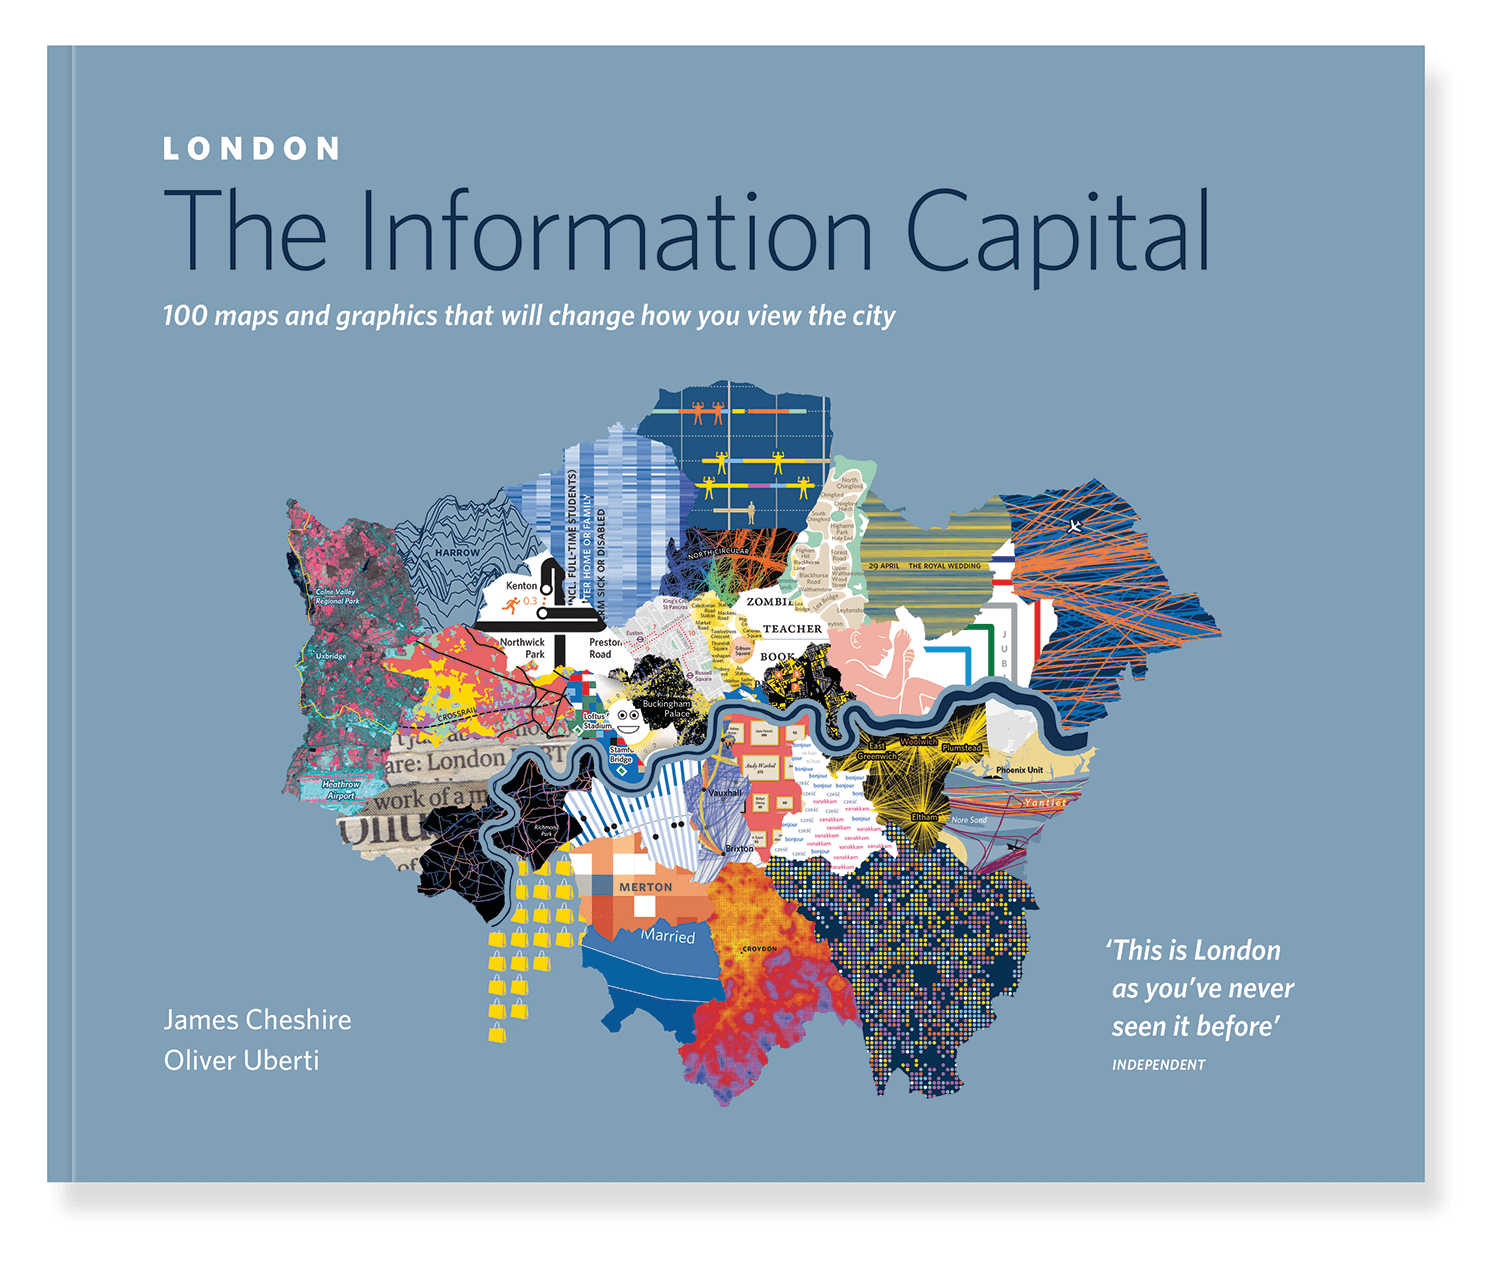
\includegraphics[width=500pt]{images/w08/information_capital} 

}

\caption{London: The Information Capital by Professor [James Cheshire](https://jcheshire.com/) and [Oliver Uberti](https://www.oliveruberti.com/the-information-capital).}\label{fig:london-information-capital}
\end{figure}

The application of quantitative research methods to data about the ``real-world'' is at the heart of this exercise. All data are collected at a single point in time and so may become out of date, or they may be too generalised to capture the minutiae of an area. Such limitations are not as significant as they once were since we now have access to data in more detail than ever before, but this does not relinquish the need to get a sense for the broader context of the study area.

\hypertarget{this-week}{%
\section*{This week}\label{this-week}}
\addcontentsline{toc}{section}{This week}

This week we will be mapping crime \textbf{hotspots} in the London boroughs of \href{https://www.google.com/maps/place/London+Borough+of+Camden,+London/@51.5428102,-0.1944449,13z/data=!3m1!4b1!4m5!3m4!1s0x48761aec186b9a3d:0x41185c626be66e0!8m2!3d51.5454736!4d-0.1627902?hl=en}{Camden} and \href{https://www.google.com/maps/place/London+Borough+of+Islington,+London/@51.5470193,-0.1444663,13z/data=!3m1!4b1!4m5!3m4!1s0x48761b5dedeb3be5:0x54f085cb18ec65c9!8m2!3d51.5465063!4d-0.1058058?hl=en}{Islington}. The data we will be working with for this week's task are downloaded from the \href{https://data.police.uk/}{data.police.uk} website. The release of official police crime data to the public was controversial at the time, with some people expressing concern that areas will have reputational damage, that the identities of victims would be revealed and that there would be social and economic consequences such as a fall in house prices in high crime areas. Others argued that the release of the data would be an important step in making the police force more accountable since the public could track whether crimes were being solved or if police are using their stop and search powers to target specific groups.

\textbf{Note}
You are expected to work through the following computer tutorial on your own, however, you need to submit your worksheet for this week as a group.

\hypertarget{getting-started}{%
\section*{Getting started}\label{getting-started}}
\addcontentsline{toc}{section}{Getting started}

Some of you may already have played around with some GIS software such as \href{https://www.arcgis.com/index.html}{ArcGIS}, but today we will be using the open-source GIS sofware suite \href{https://www.qgis.org/en/site/}{QGIS}. A copy of \href{https://www.qgis.org/en/site/}{QGIS} comes pre-installed on all cluster room computers as well as on \href{https://www.ucl.ac.uk/isd/services/computers/remote-access/desktopucl-anywhere}{Desktop@UCL Anywhere}. \href{mailto:Desktop@UCL}{\nolinkurl{Desktop@UCL}} Anywhere is a service that allows remote access to UCL resources for staff and students. All you need is a valid UCL user ID and password, an internet connection and supported web browser. Today we will be using this \href{mailto:Desktop@UCL}{\nolinkurl{Desktop@UCL}} Anywhere service. Let's get started by opening an internet browser and navigating to: \url{https://ucldesktop.cloud.com}.

\begin{figure}

{\centering \includegraphics[width=850pt]{images/w08/ucl_login} 

}

\caption{[Desktop@UCL Anywhere]((https://ucldesktop.cloud.com)) login interface.}\label{fig:ucl-desktop-login}
\end{figure}

You can login with your normal \textbf{UCL username} and \textbf{UCL password}. After this, you click on the \href{mailto:Desktop@UCL}{\nolinkurl{Desktop@UCL}} Anywhere icon to start the service:

\begin{figure}

{\centering 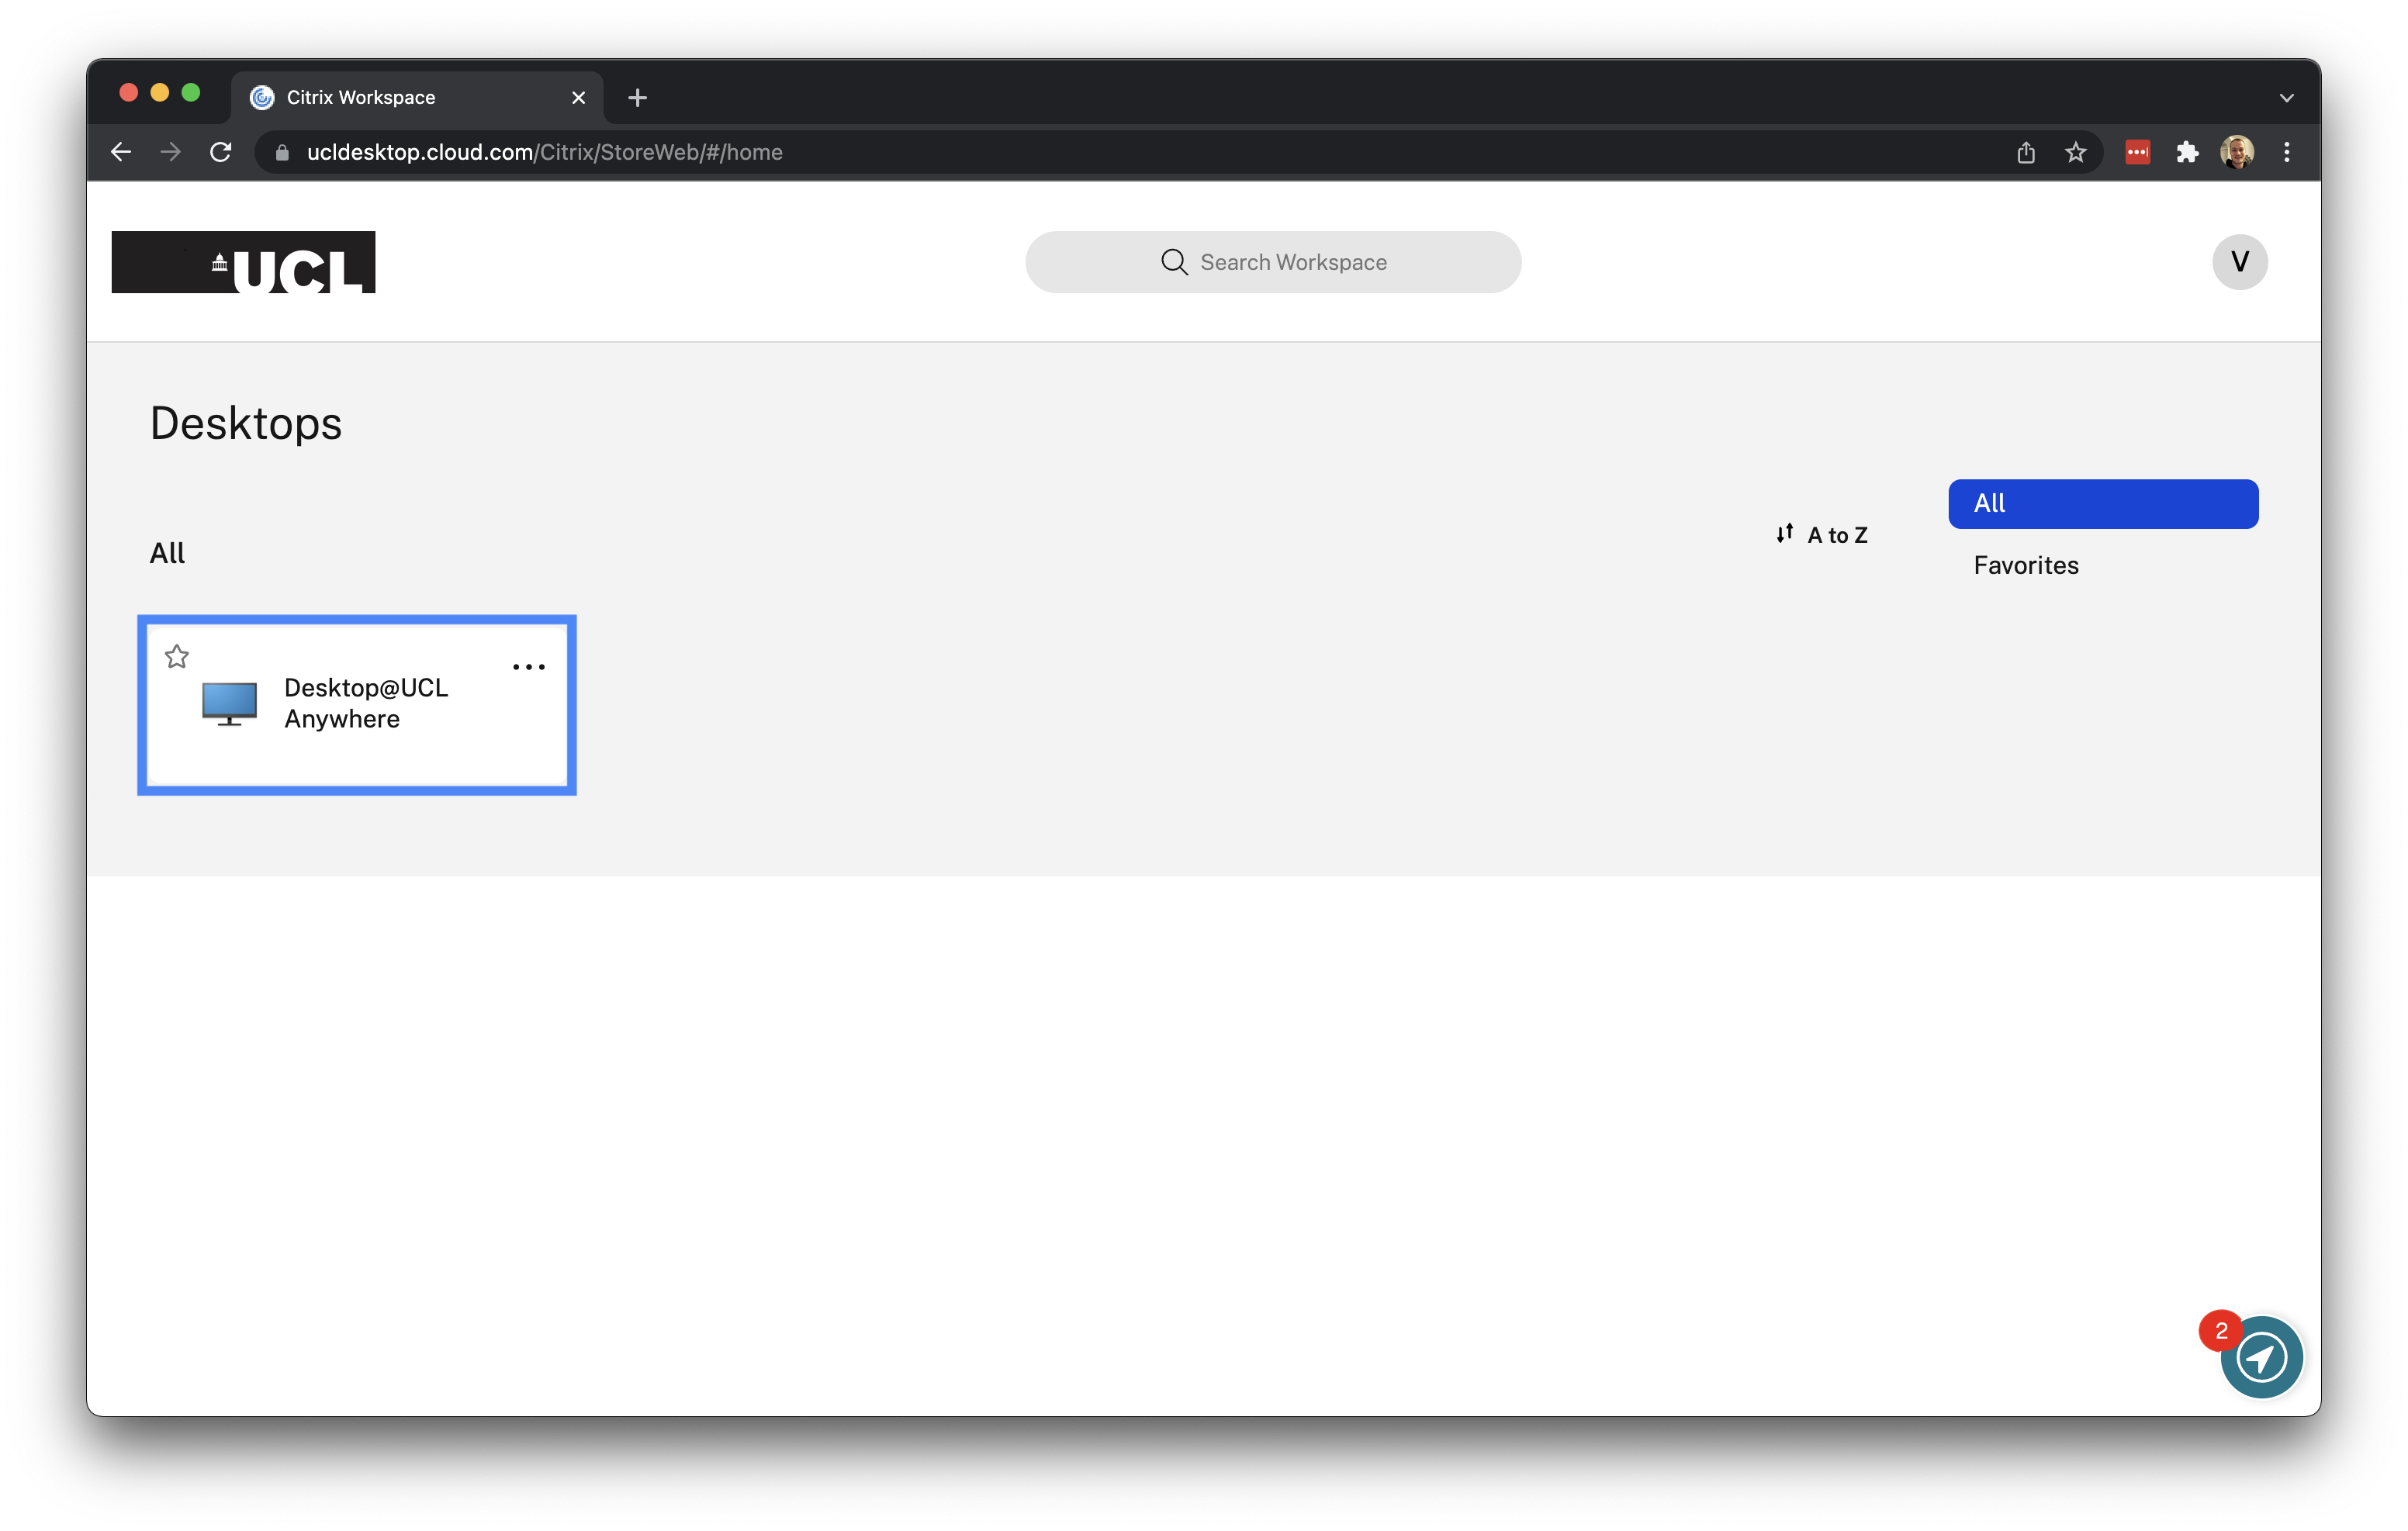
\includegraphics[width=850pt]{images/w08/ucl_start} 

}

\caption{Starting [Desktop@UCL Anywhere]((https://ucldesktop.cloud.com)).}\label{fig:ucl-desktop-start}
\end{figure}

It may take a few minutes to load, but after this you should see your normal UCL Windows desktop:

\begin{figure}

{\centering 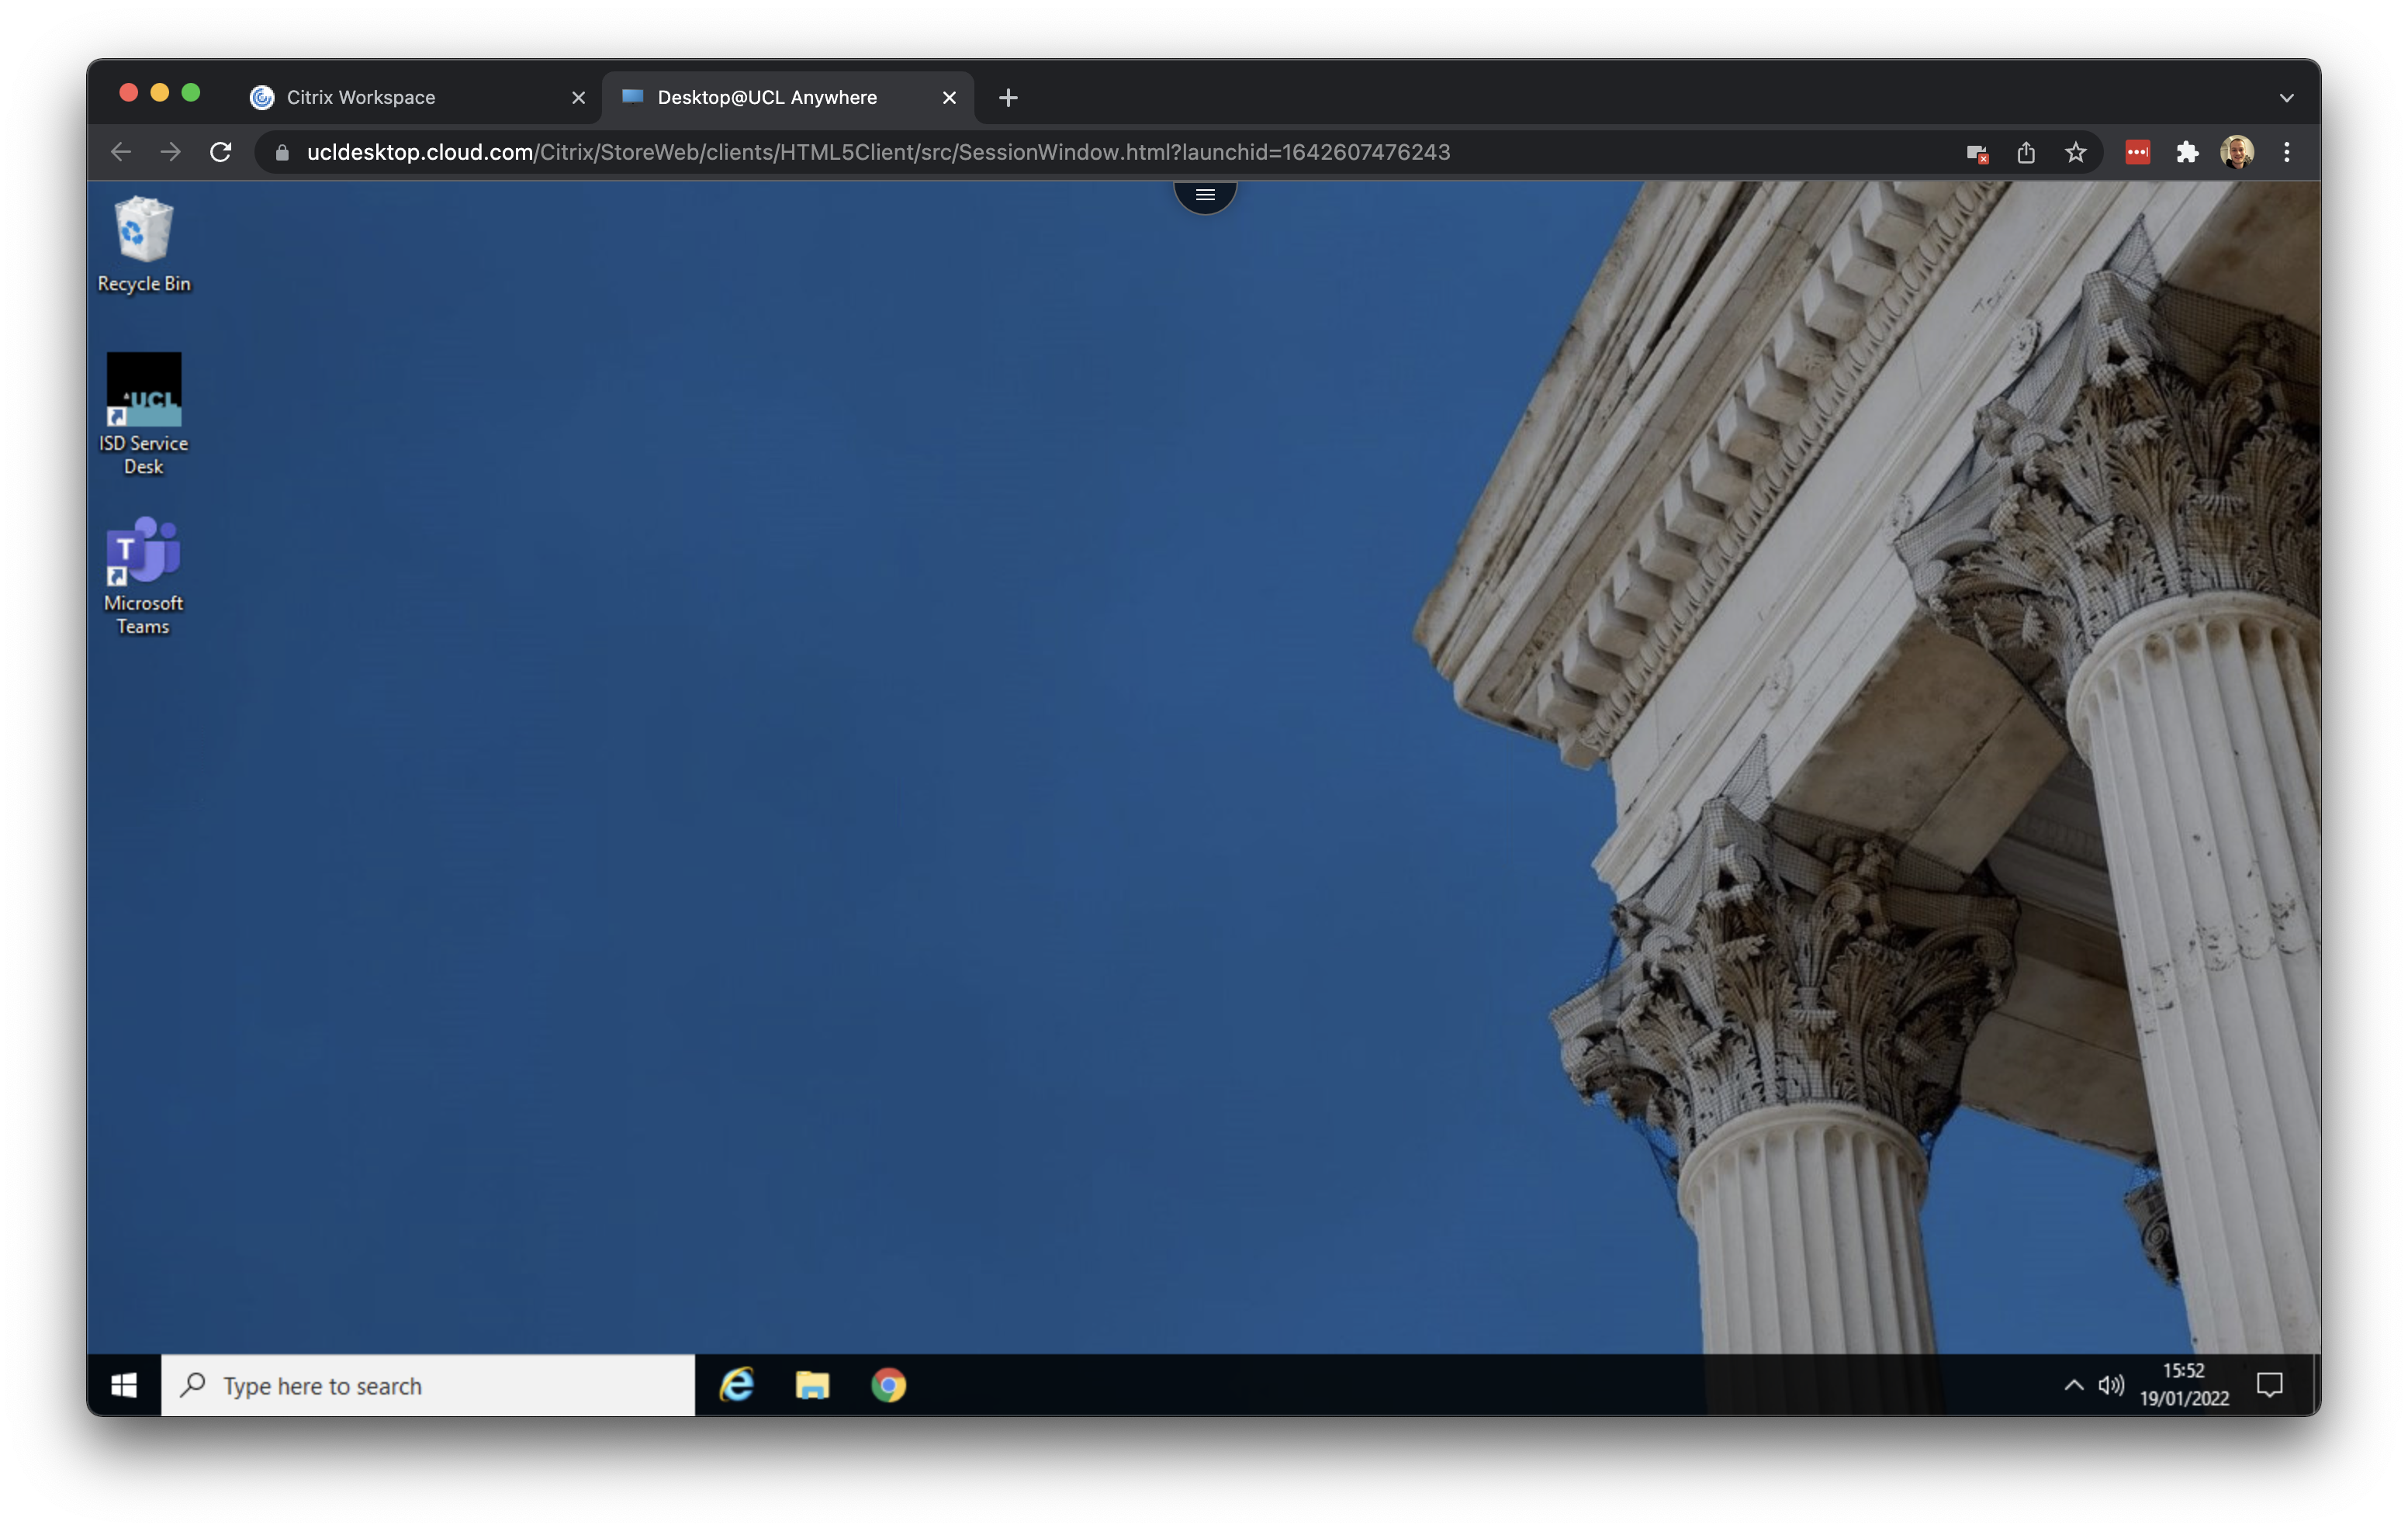
\includegraphics[width=850pt]{images/w08/ucl_login_success} 

}

\caption{Your [Desktop@UCL Anywhere]((https://ucldesktop.cloud.com)).}\label{fig:ucl-desktop-login-success}
\end{figure}

\hypertarget{downloading-crime-data}{%
\section*{Downloading crime data}\label{downloading-crime-data}}
\addcontentsline{toc}{section}{Downloading crime data}

\hypertarget{mapping-crime-data}{%
\section*{Mapping crime data}\label{mapping-crime-data}}
\addcontentsline{toc}{section}{Mapping crime data}

\hypertarget{worksheet}{%
\section*{Worksheet}\label{worksheet}}
\addcontentsline{toc}{section}{Worksheet}

Now you have worked through the steps in the computer tutorial on \protect\hyperlink{downloading-crime-data}{downloading} and \protect\hyperlink{mapping-crime-data}{mapping} crime data, you should do the following:

\textbf{Note}
You should be conducting the below steps together with your group members. You can only submit one worksheet per group.

\begin{enumerate}
\def\labelenumi{\arabic{enumi}.}
\tightlist
\item
  Using what you have learnt in the computer tutorial create two heat maps for \textbf{Camden and Islington}. The first of \textbf{anti-social behaviour} and the second of \textbf{bicycle theft}.
\item
  There are a number of crime \textbf{hot spots} for \textbf{anti-social behaviour} and \textbf{bicycle theft} that appear near UCL (particularly around Kings Cross Station). Using \href{https://www.google.com/maps/place/Kings+Cross+Station/@51.531233,-0.1265839,17z/data=!3m1!4b1!4m5!3m4!1s0x48761ba3a5a1470b:0xd5656d630ccedd8c!8m2!3d51.531233!4d-0.1243952}{Google Streetview} for context, what features distinguish them from their surrounding lower crime areas?
\item
  Using the data, zoom in on the street you have been allocated. What is the dominant type of crime on this street and its surrounding area in **December*?
\item
  Revisit the \href{https://data.police.uk/}{data.police.uk} website and create a heatmap for crime around your street in \textbf{July 2021} and \textbf{December 2021}. As there may be very few or no crimes in your allocated street, you can zoom out a little to incorporate surrounding streets. Do the patterns and dominant crime types differ over the course of the year?
\item
  Given your knowledge of your street and your observations of the crime hotspots around UCL and Kings Cross what other datasets might be useful to analyse crime in London?
\item
  Do you think the chances of falling victim of crime are higher or lower in the crime hotspots, how might you measure this?
\end{enumerate}

\hypertarget{submission}{%
\section*{Submission}\label{submission}}
\addcontentsline{toc}{section}{Submission}

Please submit your answers to the questions above in a short \textbf{group} report: no more than \textbf{500} words, a maximum of \textbf{4} maps, and \textbf{2} photographs. This is the worksheet task for the week. You can find the submission link for this final worksheet task on \href{https://moodle.ucl.ac.uk/course/view.php?id=23839}{Moodle}; one submission per group. \href{https://www.youtube.com/watch?v=h_D3VFfhvs4}{That is it for this week's Geography in the Field!}

\end{document}
